\def\leftcircle{(-1,0) circle (2 cm)}
\def\rightcircle{(1,0) circle (2 cm)}

\begin{figure}[H]
  \centering
  \label{tikzpic:set_intersection}
  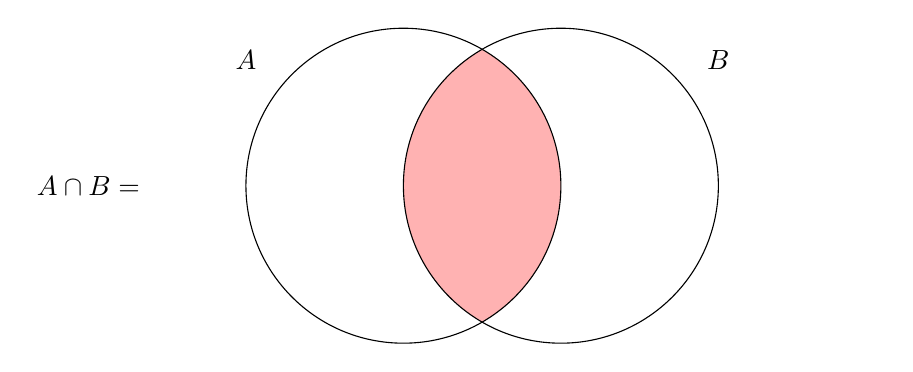
\begin{tikzpicture}
    \begin{scope}
      \clip \leftcircle;
      \fill[red!30] \rightcircle;
    \end{scope}
            
    \draw \leftcircle;
    \draw \rightcircle;
    \draw (-3,1.6) node {$A$};
    \draw (3,1.6) node {$B$};
    \draw (-5,0) node {$A \cap B = $};
    \draw (5,0) node {\text{     }};
  \end{tikzpicture}
  \caption{Пересечение множеств}
\end{figure}

